\documentclass[12pt,fleqn]{article}\usepackage{../../common}
\begin{document}
Tam Diferansiyel (Total Differential)

Bir $f$ fonksiyonunun tam diferansiyeli (total differential) o
fonksiyonun lineerleştirilmesi anlamına gelir. İki değişkenli bir
fonksiyon için şöyle temsil edilir:

$$ df = f_x(x_0, y_0)dx + f_y(x_0,y_0)dy  $$

Bu formu nasıl türetiriz? Bize lazım olan lineerleştirme formülasyonu. Tek
değişkenli bir fonksiyonu lineerleştirmenin tekniği şudur:

$$ L(x) = f(x_0) + f'(x_0) \Delta x  $$

Burada $L(x)$ gerçek fonksiyonu yaklaşıksal (approximate) olarak temsil eden
lineer fonksiyondur. 

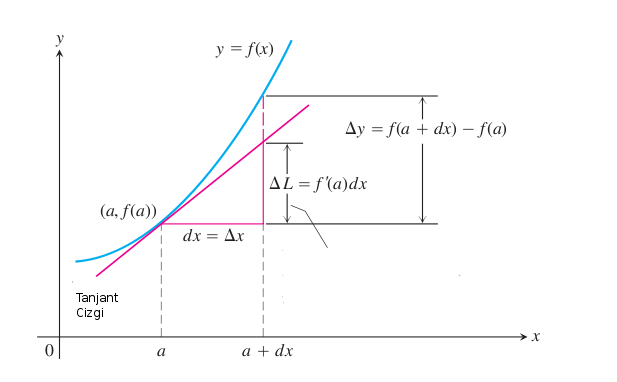
\includegraphics[height=6cm]{calc_multi_app_06.png}

Bu fonksiyonu genişleterek iki değişkenli hale getirelim (sadece $y$
ekleyeceğiz)

$$ L(x,y) = f(x_0,y) + f_x(x_0,y) \Delta x $$

Bu fonksiyon da bir önceki kadar ``geçerli''. Sonuçta fonksiyonlar
noktasal değerlere göre sonuç verirler, bu sebeple bir lineerleştirme
işlemi 2 boyutlu ortamda herhangi bir $x$ noktasında yapılabildiği
gibi, herhangi bir $x$, $y$ noktasında da yapılabilir.

Şimdi üstteki denklemin sağ tarafında yer alan $f(x_0,y)$'yi lineerleştirelim.  

$$ L(x,y) = L(x_0,y_0) + f_y(x_0,y_0) \Delta y + f_x(x_0,y_0) \Delta x $$

Artık $L(x_0,y_0)$'yi sol tarafa taşıyabiliriz:

$$ \Delta L = L(x,y) - L(x_0,y_0) = f_y(x_0,y_0) \Delta y + f_x(x_0,y_0)
\Delta x $$ 

$\Delta L$ yani $df$ istediğimiz tam diferensiyel sonucudur, $\Delta
x$ yerine $dx$, $\Delta y$ yerine $dy$ kullanabiliriz, o zaman baştaki
formun aynısını elde etmiş oluruz.

Türetirken kullandığımız numarayı üç, dört, vs. gibi istediğimiz kadar
değişken taşıyan $f$ fonksiyonları için yapabilirdik, ve sonuç üstteki
forma benzer olurdu. Her değişkenin kısmi türevi o değişkenin sonsuz
ufaklıktaki ``değişimi'' ile çarpılıp, o çarpımlar toplanınca elimize
tam diferansiyel geçiyor.

Bu yazı [1, sf. 130], [1, sf. 347], [1, sf. 358], ve [1, sf. 257]'yi baz
almıştır. Diğer kaynaklar altta. 

Kaynaklar

[1] Thomas, {\em Thomas Calculus 11th Edition}


\end{document}
